\subsection{Mixer, Oscillator, Frequency Conversion}
\label{subsec:mixer-osc}

In this section, we'll dive into the fascinating world of mixers, oscillators, and frequency conversion. These components are the hidden champions of radio technology, quietly working behind the scenes to make sure your signals get where they need to go. Let's break it down, shall we?

\subsubsection*{The Role of a Mixer}

A mixer is like the DJ of the radio world—it takes two signals and blends them together to create something new. Specifically, a mixer performs frequency conversion, which is essential for shifting signals from one frequency to another. This is crucial in radio systems because it allows us to transmit and receive signals at different frequencies without interference.

Imagine you have a signal at frequency \( f_1 \) and you want to convert it to frequency \( f_2 \). The mixer takes this signal and combines it with another signal from a local oscillator (more on that later) at frequency \( f_{LO} \). The result is a new signal at the sum or difference of these frequencies, typically \( f_1 + f_{LO} \) or \( f_1 - f_{LO} \). This process is known as heterodyning, and it's the backbone of frequency conversion in radio systems.





\subsubsection*{The Function of an Oscillator}

Now, let's talk about the oscillator. If the mixer is the DJ, the oscillator is the beat generator. It produces a signal at a specific frequency, which is then used by the mixer to perform frequency conversion. Oscillators are also key players in frequency synthesis and modulation, where they help generate the precise frequencies needed for various radio applications.

An oscillator circuit typically consists of an amplifier and a feedback loop that sustains the oscillation. The frequency of the output signal is determined by the components in the circuit, such as capacitors and inductors. This makes oscillators incredibly versatile, as they can be tuned to produce a wide range of frequencies. We will cover oscillators in more detail in upcoming books of this series. For now, just remember that an oscillator is a circuit that generates a signal at a specific frequency.


\subsubsection*{Frequency Conversion: The Big Picture}

Frequency conversion is the process of changing a signal's frequency, and it's where mixers and oscillators come together in perfect harmony. The mixer takes the input signal and the oscillator's signal, and through the magic of heterodyning, produces a new signal at the desired frequency. This is essential in radio systems, where signals often need to be shifted to different frequencies for transmission, reception, or further processing.

For example, in a superheterodyne receiver, the incoming signal is mixed with a local oscillator signal to produce an intermediate frequency (IF) that's easier to process. This allows the receiver to be more selective and sensitive, improving overall performance.


\begin{table}[h!]
    \centering
    \begin{tabular}{|l|l|}
        \hline
        \textbf{Component} & \textbf{Function} \\
        \hline
        Mixer & Performs frequency conversion by combining input signals with a local oscillator signal. \\
        Oscillator & Generates a signal at a specific frequency for use in frequency conversion and modulation. \\
        \hline
    \end{tabular}
    \caption{Mixer and Oscillator Functions}
    \label{tab:mixer-oscillator}
\end{table}

\subsubsection*{Questions}

\begin{tcolorbox}[colback=gray!10!white,colframe=black!75!black,title={T7A03}]
    Which of the following is used to convert a signal from one frequency to another?
    \begin{enumerate}[label=\Alph*),noitemsep]
        \item Phase splitter
        \item \textbf{Mixer}
        \item Inverter
        \item Amplifier
    \end{enumerate}
\end{tcolorbox}

A mixer is used to convert a signal from one frequency to another by combining it with a local oscillator signal. This process is known as heterodyning. The other options—phase splitter, inverter, and amplifier—do not perform frequency conversion.

\begin{tcolorbox}[colback=gray!10!white,colframe=black!75!black,title={T7A05}]
    What is the name of a circuit that generates a signal at a specific frequency?
    \begin{enumerate}[label=\Alph*),noitemsep]
        \item Reactance modulator
        \item Phase modulator
        \item Low-pass filter
        \item \textbf{Oscillator}
    \end{enumerate}
\end{tcolorbox}

An oscillator is a circuit that generates a signal at a specific frequency. Reactance modulators, phase modulators, and low-pass filters do not generate signals at specific frequencies; they modify or filter existing signals.

\begin{figure}[h]
    \centering
    \footnotesize
    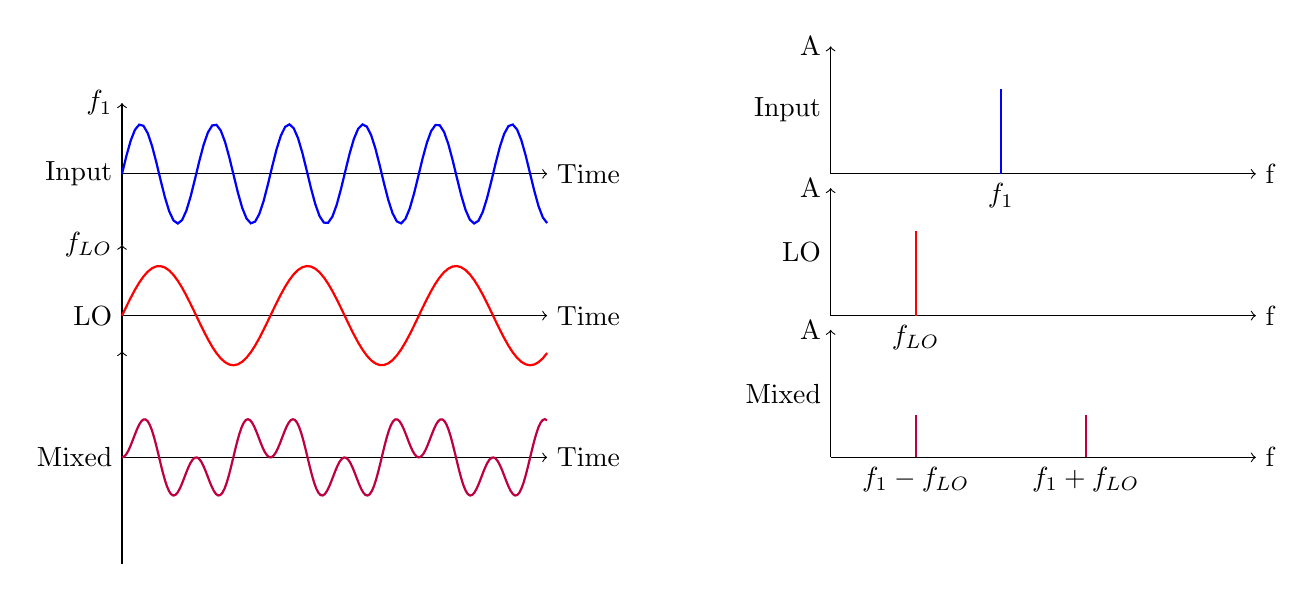
\begin{tikzpicture}[scale=0.9]
        % Grid settings
        \def\gridXmin{0}
        \def\gridXmax{6}
        \def\gridYmin{-4}
        \def\gridYmax{4}
        
        % Time Domain Plots (Left Side)
        % Input Signal
        \begin{scope}[shift={(0,2)}]
            \draw[->] (\gridXmin,0) -- (\gridXmax,0) node[right] {Time};
            \draw[->] (0,-1) -- (0,1) node[left] {$f_1$};
            \draw[blue, thick] plot[domain=0:6,samples=100] 
                (\x,{0.7*sin(6*\x r)});
            \node[left] at (0,0) {Input};
        \end{scope}
        
        % LO Signal
        \begin{scope}[shift={(0,0)}]
            \draw[->] (\gridXmin,0) -- (\gridXmax,0) node[right] {Time};
            \draw[->] (0,-1) -- (0,1) node[left] {$f_{LO}$};
            \draw[red, thick] plot[domain=0:6,samples=100] 
                (\x,{0.7*sin(3*\x r)});
            \node[left] at (0,0) {LO};
        \end{scope}
        
        % Mixed Output
        \begin{scope}[shift={(0,-2)}]
            \draw[->] (\gridXmin,0) -- (\gridXmax,0) node[right] {Time};
            \draw[->] (0,-1.5) -- (0,1.5) node[above] {};
            \draw[purple, thick] plot[domain=0:6,samples=200] 
                (\x,{0.7*sin(6*\x r)*sin(3*\x r)});
            \node[left] at (0,0) {Mixed};
        \end{scope}
        
        % Frequency Domain Plots (Right Side)
        % Input Spectrum - widened scale
        \begin{scope}[shift={(10,2)}, scale=1.2]    % Increased scale from 0.8 to 1.2
            \draw[->] (0,0) -- (5,0) node[right] {f};    % Increased width from 4 to 5
            \draw[->] (0,0) -- (0,1.5) node[left] {A};  % Adjusted height
            \draw[blue, thick] (2,0) -- (2,1);
            \node[below] at (2,0) {$f_1$};
            \node[left] at (0,0.75) {Input};
        \end{scope}
        
        % LO Spectrum
        \begin{scope}[shift={(10,0)}, scale=1.2]
            \draw[->] (0,0) -- (5,0) node[right] {f};
            \draw[->] (0,0) -- (0,1.5) node[left] {A};
            \draw[red, thick] (1,0) -- (1,1);
            \node[below] at (1,0) {$f_{LO}$};
            \node[left] at (0,0.75) {LO};
        \end{scope}
        
        % Output Spectrum
        \begin{scope}[shift={(10,-2)}, scale=1.2]
            \draw[->] (0,0) -- (5,0) node[right] {f};
            \draw[->] (0,0) -- (0,1.5) node[left] {A};
            \draw[purple, thick] (1,0) -- (1,0.5);
            \draw[purple, thick] (3,0) -- (3,0.5);
            \node[below] at (1,0) {$f_1 - f_{LO}$};
            \node[below] at (3,0) {$f_1 + f_{LO}$};
            \node[left] at (0,0.75) {Mixed};
        \end{scope}
    \end{tikzpicture}
    \caption{Signal Mixing Process: Shows both time domain (left) and frequency domain (right) representations of the mixing process. The mixer multiplies the input signal ($f_1$) with the local oscillator signal ($f_{LO}$), producing sum ($f_1 + f_{LO}$) and difference ($f_1 - f_{LO}$) frequencies in the output. The time domain shows the actual waveforms, while the frequency domain shows the spectral components.}
    \label{fig:mixing-process}
\end{figure}
